\chapter{Dokumenty odkazované z textu}
\begin{figure*}[ht]
    \centering
   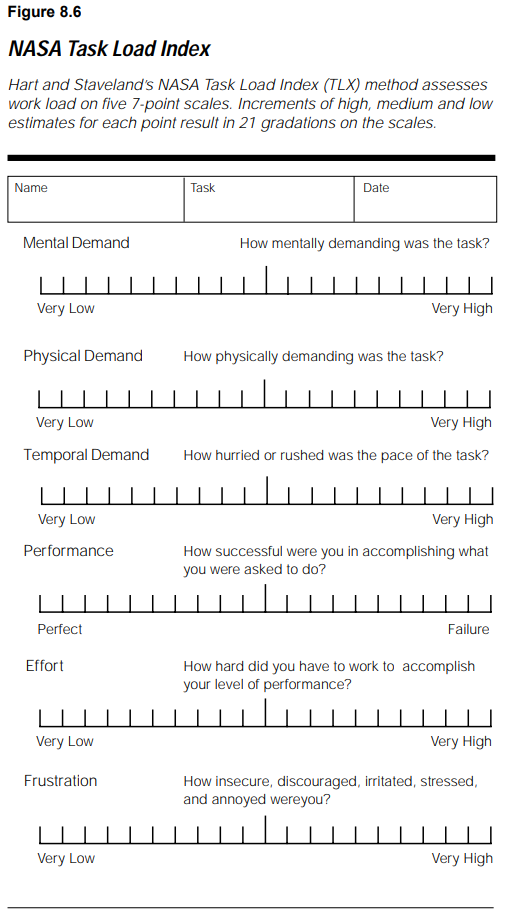
\includegraphics[width=0.78\linewidth]{obrazky-figures/nasaTLXform.png}
  \caption{NASA TLX (Task Load Index) - formulář pro subjektivní posouzení pracovní zátěže. Převzato z \cite{NasaTlx}.}
  \label{pic-nasaTlxForm}
\end{figure*}
\chapter{Paměťové médium}
Přiložené paměťové médium obsahuje zdrojové kódy rozhraní, propagační fotografie/videa a zdrojové kódy práce pro vytvoření PDF dokumentu.
\section{Demonstrační video}
Dle zadání vytvořené propagační video demonstrující klíčové vlastnosti řešení.
\section{Zdrojové kódy}
Médium obsahuje kompletní zdrojové kódy řešení včetně potřebných knihoven pro kompilaci a spuštění. Jsou zde přítomné i kódy pro vytvoření textové části práce.
\section{Shrnující plakát s přiloženým komentářem}
Plakát je ve formátu A1 a obsahuje souhrn informací o řešení.